\begin{name}
	{NGUYÊN HÀM - TÍCH PHÂN}
	{KT ỨNG DỤNG NGUYÊN HÀM - TÍCH PHÂN}
	{\tentruong}
	{\thoigian}
\end{name}
\setcounter{ex}{0}\setcounter{bt}{0}
\Opensolutionfile{ans}[ans/ans-2-B13-1]
\caulc
%Câu 1
\begin{ex}%[2D4N3-1]
	Cho hàm số $y=f(x)$ liên tục trên đoạn $[a;b]$. Viết công thức tính diện tích $S$ của hình phẳng giới hạn bởi đồ thị hàm số đã cho, trục hoành và hai đường thẳng $x=a$, $x=b$ $(a<b)$.
	\choice
	{\True $S=\displaystyle\int\limits_a^b |f(x)|\mathrm{\,d}x$}
	{$S=\displaystyle\int\limits_a^b [f(x)]^2\mathrm{\,d}x$}
	{$S=\displaystyle\int\limits_b^a |f(x)|\mathrm{\,d}x$}
	{$S=\displaystyle\int\limits_a^b f(x)\mathrm{\,d}x$}
	\loigiai{
	Diện tích $S$ của hình phẳng giới hạn bởi đồ thị hàm số đã cho, trục hoành và hai đường thẳng $x=a$, $x=b$ $(a<b)$ là $S=\displaystyle\int\limits_a^b |f(x)|\mathrm{\,d}x$.
	}
\end{ex}
%Câu 2
\begin{ex}%[2D4N3-4]
	Trong không gian $Oxyz$, vật thể $(H)$ giới hạn bởi hai mặt phẳng có phương trình $x=a$ và $x=b$ với $a<b$. Gọi $S(x)$ là diện tích thiết diện của $(H)$ bị cắt bởi mặt phẳng vuông góc với trục $Ox$ tại điểm có hoành độ là $x$ với $a\le x\le b$. Giả sử hàm số $S(x)$ liên tục trên đoạn $[a;b]$. Khi đó, thể tích $V$ của vật thể $(H)$ được tính bởi công thức
	\choice
	{$V=\pi\displaystyle\int\limits_a^bS(x)\mathrm{\,d}x$}
	{\True $V=\displaystyle\int\limits_a^bS(x)\mathrm{\,d}x$}
	{$V=\displaystyle\int\limits_a^bS^2(x)\mathrm{\,d}x$}
	{$V=\pi\displaystyle\int\limits_a^bS^2(x)\mathrm{\,d}x$}
	\loigiai{
	Ta có $V=\displaystyle\int\limits_a^bS(x)\mathrm{\,d}x$.
	}
\end{ex}
%Câu 3
\begin{ex}%[2D4H3-1]
	\immini{Cho hàm số $ y=f(x) $ liên tục trên $ \mathbb{R} $ và có đồ thị như hình vẽ bên. Gọi $ S $ là diện tích hình phẳng được giới hạn bởi đồ thị hàm số $ y=f(x) $ và trục hoành. Khẳng định nào sau đây đúng?
	\choice
	{$ \displaystyle\int\limits_{-1}^{0} f(x)\mathrm{\,d}x-\displaystyle\int\limits_{0}^{2} f(x)\mathrm{\,d}x $}
	{\True $ -\displaystyle\int\limits_{-1}^{0} f(x)\mathrm{\,d}x+\displaystyle\int\limits_{0}^{2} f(x)\mathrm{\,d}x $}
	{$ \displaystyle\int\limits_{-1}^{0} f(x)\mathrm{\,d}x+\displaystyle\int\limits_{0}^{2} f(x)\mathrm{\,d}x $}
	{$ -\displaystyle\int\limits_{-1}^{0} f(x)\mathrm{\,d}x-\displaystyle\int\limits_{0}^{2} f(x)\mathrm{\,d}x $}}{\begin{tikzpicture}[scale=0.7,>=stealth, font=\footnotesize, line join=round, line cap=round]
	\draw[->] (-2,0)--(3,0) node [below]{$x$};
	\draw[->] (0,-1.3)--(0,4) node [left]{$y$};
	\draw[fill=black] (0,0)circle (1pt)node [above left]{$O$};
	\clip (-2,-2.5) rectangle (3,3);
	\draw[smooth,samples=300,domain=-2:2.2] plot(\x,{-1*(\x+1)*(\x-0)*(\x-2)})node[left]{$ $};
	\fill[pattern=north east lines,opacity=0.8] plot[domain=-1:0](\x,{-1*(\x+1)*(\x-0)*(\x-2)})--cycle;
	\fill[pattern=north east lines,opacity=0.8] plot[domain=0:2](\x,{-1*(\x+1)*(\x-0)*(\x-2)})--cycle;
	\foreach \x/\g in{-1/250,2/-100}
	\draw[fill=black](\x,0)circle(1pt)node[shift={(\g:0.35)}]{$\x$};
	\end{tikzpicture}}
	\loigiai{
	Từ đồ thị ta được $S= -\displaystyle\int\limits_{-1}^{0} f(x)\mathrm{\,d}x+\displaystyle\int\limits_{0}^{2} f(x)\mathrm{\,d}x $.
	}
\end{ex}
%Câu 4
\begin{ex}%[2D4N3-3]
	Cho hình phẳng giới hạn bởi đồ thị của hàm số $ y=f(x)$ liên tục và không âm trên đoạn $\left[1;3\right]$, trục $ Ox$ và hai đường thẳng $ x=1$, $x=3$ quay quanh trục $ Ox$, ta được khối tròn xoay. Thể tích của khối tròn xoay này được tính theo công thức nào dưới đây?
	\choice
	{$V=\displaystyle\int\limits_1^3f(x)\mathrm{\,d}x$}
	{$V=\displaystyle\int\limits_1^3\left[f(x)\right]^2\mathrm{\,d}x$}
	{$V=\pi\displaystyle\int\limits_1^3f(x)\mathrm{\,d}x$}
	{\True $V=\pi\displaystyle\int\limits_1^3\left[f(x)\right]^2\mathrm{\,d}x$}
	\loigiai{
	Ta có $V=\pi\displaystyle\int\limits_1^3\left[f(x)\right]^2\mathrm{\,d}x$.
	}
\end{ex}
%Câu 5
\begin{ex}%[2D4H3-1]
	Tính diện tích $S$ hình phẳng giới hạn bởi các đường $y=2x^2$, $y=-1$, $x=0$ và $x=1$.
	\choice
	{$S=\dfrac{1}{3}$}
	{\True $S=\dfrac{5}{3}$}
	{$S=\dfrac{47}{15}$}
	{$S=\dfrac{5\pi}{3}$}
	\loigiai{
	Ta có $S=\displaystyle\int\limits_0^1|2x^2-(-1)|\mathrm{\,d}x=\displaystyle\int\limits_0^1(2x^2+1)\mathrm{\,d}x=\left(\dfrac{2x^3}{3}+x\right)\bigg|_0^1=\dfrac{5}{3}$.
	}
\end{ex}
%Câu 6
\begin{ex}%[2D4H3-3]
	Cho hình phẳng $(S)$ giới hạn bởi $Ox$ và $y=\sqrt{1-x^2}$. Thể tích khối tròn xoay khi quay $(S)$ quanh trục $Ox$ là
	\choice
	{$\dfrac{3}{2}\pi $}
	{$\dfrac{2}{3}\pi $}
	{\True $\dfrac{4}{3}\pi $}
	{$\dfrac{3}{4}\pi $}
	\loigiai{
	Phương trình hoành độ giao điểm của đường $y=\sqrt{1-x^2}$ và trục $Ox$ $$\sqrt{1-x^2}=0\Leftrightarrow\hoac{&x=1\\&x=-1.}$$
	Thể tích khối tròn xoay là $V=\pi\displaystyle\int\limits_{-1}^{1} y^2\mathrm{\,d}x=\pi\displaystyle\int\limits_{-1}^{1}(1-x^2)\mathrm{\,d}x=\dfrac{4}{3}\pi$.
	}
\end{ex}
%Câu 7
\begin{ex}%[2D4H3-4]
	Tính thể tích $V$ của phần vật thể giới hạn bởi hai mặt phẳng $x=1$ và $x=3$, biết rằng khi cắt vật thể bởi mặt phẳng vuông góc với trục $Ox$ tại điểm có hoành độ $x$ ($1\le x\le 3$) thì được thiết diện là một hình chữ nhật có độ dài hai cạnh là $3x$ và $\sqrt{3x^2-2}$.
	\choice
	{$V=(32+2\sqrt{15})\pi$}
	{\True $V=\dfrac{124}{3}$}
	{$V=\dfrac{124\pi}{3}$}
	{$V=32+2\sqrt{15}$}
	\loigiai{
	Diện tích thiết diện là $S(x)=3x\cdot \sqrt{3x^2-2}$.\\
	Thể tích vật thể là
	$$V=\displaystyle\int\limits_1^3 S(x) \mathrm{\,d}x=\displaystyle\int\limits_1^3 3x\sqrt{3x^2-2} \mathrm{\,d}x.$$
	Đặt $t=\sqrt{3x^2-2}\Rightarrow t^2=3x^2-2\Rightarrow t \mathrm{\,d}t=3x \mathrm{\,d}x$.\\
	Đổi cận $x=1\Rightarrow t=1$, $x=3\Rightarrow t=5$.\\
	Khi đó, $V=\displaystyle\int\limits_1^5 t\cdot t \mathrm{\,d}t=\dfrac{t^3}{3}\Big|_1^5=\dfrac{5^3}{3}-\dfrac{1^3}{3}=\dfrac{124}{3}$.
	}
\end{ex}
%Câu 8
\begin{ex}%[2D4H3-1]
	Diện tích hình phẳng giới hạn bởi các đường cong $y=x^3-6x$ và $y=x^2$ bằng
	\choice
	{$\dfrac{125}{12}$}
	{$\dfrac{16}{3}$}
	{$\dfrac{63}{4}$}
	{\True $\dfrac{253}{12}$}
	\loigiai
	{
	Xét phương trình hoành độ giao điểm của hai đường cong đã cho $$x^3-6x=x^2\Leftrightarrow x\left (x^2-x-6 \right )=0\Leftrightarrow\hoac{& x=0\\&x=-2\\&x=3 .}$$
	Diện tích hình phẳng cần tìm là
	\allowdisplaybreaks
	\begin{eqnarray*}
	S&=&\displaystyle\int\limits_{-2}^{3}\left |x^3-6x-x^2 \right |\mathrm{\,d}x\\
	&=&\displaystyle\int\limits_{-2}^{0}\left |x^3-6x-x^2 \right |\mathrm{\,d}x+\displaystyle\int\limits_{0}^{3}\left |x^3-6x-x^2 \right |\mathrm{\,d}x\\
	&=&\displaystyle\int\limits_{-2}^{0}\left(x^3-6x-x^2 \right)\mathrm{\,d}x+\displaystyle\int\limits_{0}^{3}\left(-x^3+6x+x^2 \right)\mathrm{\,d}x\\
	&=&\dfrac{16}{3}+\dfrac{63}{4}=\dfrac{253}{12}.
	\end{eqnarray*}
	}
\end{ex}
%Câu 9
\begin{ex}%[2D4H3-3]
	Cho hình phẳng giới hạn bởi hai đường $y=2x-x^2$ ,$y=x$. Tính thể tích khối tròn xoay thu được khi quay hình phẳng quanh trục $Ox$.
	\choice
	{$\dfrac{\pi}{6}$}
	{$\dfrac{6\pi}{5}$}
	{\True $\dfrac{\pi}{5}$}
	{$\dfrac{\pi}{25}$}
	\loigiai{
	Xét phương trình hoành độ giao điểm
	$$2x-x^2=x\Leftrightarrow -x^2+x=0\Leftrightarrow \hoac{&x=0\\&x=1.}$$
	Thể tích khối tròn xoay khi quay hình phẳng quanh trục $Ox$ là
	\begin{eqnarray*}
	V & = & \pi \displaystyle\int\limits_0^1 |(2x-x^2)^2-x^2|\mathrm{\,d}x\\
	& = & \pi \displaystyle\int\limits_0^1 |4x^2-4x^3+x^4-x^2|\mathrm{\,d}x\\
	& = & \pi \displaystyle\int\limits_0^1 |3x^2-4x^3+x^4|\mathrm{\,d}x\\
	& = & \dfrac{\pi}{5}.
	\end{eqnarray*}
	}
\end{ex}
%Câu 10
\begin{ex}%[2D4H3-1]
	\immini{
	Cho hàm số $y = f(x)$ liên tục trên $\mathbb{R}$. Gọi $S_1$; $S_2$ là diện tích của hình phẳng tương ứng như trong hình vẽ. Biết $S_1 = 4$ và $S_2 = \dfrac{4}{3}$. Tính $I=\displaystyle\int\limits_{1}^{6}f(x)\mathrm{\,d}x$.
	\choice
	{$I = \dfrac{11}{3}$}
	{$I = \dfrac{16}{3}$}
	{\True $I = \dfrac{8}{3}$}
	{$I = \dfrac{10}{3}$}
	}{
	\begin{tikzpicture}[scale=0.8, font=\footnotesize, line join=round, line cap=round, >=stealth]
	\def\xt{-0.5} \def\xp{7} \def\yt{2.5} \def\yd{-1.5}
	\draw[->] (\xt,0)--(\xp,0) node [below]{$x$};
	\draw[->] (0,\yd)--(0,\yt) node [left]{$y$};
	\node at (0,0) [below left]{$O$} circle (1pt);
	\foreach \x in {2,3,4}{
	\draw (\x,0) node[below]{$\x$} circle (1pt);
	}
	\draw (1,0) node[below left]{$1$} circle (1pt);
	\draw (5,0) node[above]{$5$} circle (1pt);
	\draw (6.05,0) node[below right]{$6$} circle (1pt);
	\draw (6.5,1.5) node[left]{$y=f(x)$};
	\foreach \x in {-1,1,2}{
	\draw (0,\x) node[left]{$\x$} circle (1pt);
	}
	\clip (\xt,\yd) rectangle (\xp,\yt);
	\draw [thick, domain=0.5:6.8, samples=100] %
	plot (\x, {0.23786*(\x)^3-2.62856*(\x)^2 + 8.14782*(\x)-5.75712});
	\draw[pattern = north east lines, pattern color = gray!60, line width = 2pt,draw=none] (1,0)%
	plot[domain=1:6] (\x, {0.23786*(\x)^3-2.62856*(\x)^2 + 8.14782*(\x)-5.75712})--(6,0)--cycle;
	\draw (2.8,0.9) node[left]{$S_1$};
	\draw (5.5,-0.5) node[left]{$S_2$};
	\end{tikzpicture}
	}
	\loigiai{
	Ta có $I = \displaystyle\int\limits_{1}^{6}f(x)\mathrm{\,d}x = \int\limits_{1}^{4}f(x)\mathrm{\,d}x+\int\limits_{4}^{6}f(x)\mathrm{\,d}x = S_1-S_2 = 4-\dfrac{4}{3} = \dfrac{8}{3}$.
	}
\end{ex}
%Câu 11
\begin{ex}%[2D4V3-1]
	\immini
	{Cho hình phẳng $(H)$ giới hạn bởi các đường $y=f(x)=\sqrt{x}$, $y=g(x)=x-2$ và trục hoành (như hình vẽ). Tính thể tích $V$ của khối tròn xoay tạo thành khi quay hình $(H)$ quanh trục hoành.
	\choice
	{$V=\dfrac{8\pi}{3}$}
	{\True $V=\dfrac{16\pi}{3}$}
	{$V=8\pi$}
	{$V=10\pi$}
	}
	{
	\begin{tikzpicture}[scale=.8,font=\footnotesize, line join=round, line cap=round, >=stealth]
	\draw[->] (-1,0) -- (5,0) node[below] {\footnotesize $x$};
	\draw[->] (0,-1) -- (0,3.5) node[left] {\footnotesize $y$};
	\coordinate[label=below left:$O$](O) at (0,0);
	\draw[samples=100,color=black,domain=0:4.5] plot (\x,{(\x)^0.5});
	\draw[color=black, domain=1.5:4.5] plot (\x,{\x-2});
	\draw (0.7,1.7) node[right]{\footnotesize $y=\sqrt{x}$};
	\draw (3,1) node[right]{\footnotesize $y=x-2$};
	\draw (2,0) node[below] {\footnotesize $2$};
	\draw [draw=none, pattern = north west lines, pattern color=black, samples=100] plot[domain=0:4] (\x,{(\x)^0.5})--(2,0)--(0,0)-- cycle;
	\foreach \diem in {O}\fill (\diem)circle(1.5pt);
	\end{tikzpicture}
	}
	\loigiai{
	Xét phương trình hoành độ giao điểm
	\[\sqrt{x}=x-2\Leftrightarrow \heva{& x\ge 2 \\ & x=(x-2)^2}\Leftrightarrow \heva{& x\ge 2 \\ & x^2-5x+4=0}\Leftrightarrow \heva{& x\ge 2 \\ & \hoac{& x=1 \\ & x=4}}\Leftrightarrow x=4.\]
	Thể tích $V$ khi cho hình phẳng $(H)$ quay quanh trục hoành là
	\[V=\pi \displaystyle\int\limits_{0}^{4} \left(\sqrt{x}\right)^2 \mathrm{\,d}x-\pi \displaystyle\int\limits_{2}^{4} \left(x-2\right)^2 \mathrm{\,d}x=\pi \cdot \dfrac{x^2}{2} \bigg|_0^4- \pi \cdot \dfrac{\left(x-2\right)^3}{3}\bigg|_2^4=\dfrac{16\pi}{3}.\]
	}
\end{ex}
%Câu 12
\begin{ex}%[2D4V3-2]
	\immini{
	Một mảnh đất hình chữ nhật có chiều dài $60$ m, chiều rộng $20$ m. Người ta muốn trồng cỏ ở hai đầu của mảnh đất hai hình bằng nhau giới hạn bởi hai đường Parabol có hai đỉnh cách nhau $40$ m (như hình vẽ bên). Phần còn lại của mảnh đất người ta lát gạch với chi phí là $200\,000$ đồng/m$^2$. Tính tổng số tiền để lát gạch (làm tròn đến hàng nghìn).
	\choice
	{$133\,334\,000$ đồng}
	{$186\,667\,000$ đồng}
	{$53\,334\,000$ đồng}
	{\True $213\,334\,000$ đồng}
	}
	{
	\begin{tikzpicture}[font=\footnotesize, line join=round, line cap=round, >=stealth,scale=1.2]
	\path (-1,1) coordinate (A)
	(1,1) coordinate (B)
	(-1,-3) coordinate (C)
	(1,-3) coordinate (D)
	(-1.3,0) coordinate (F)
	(-1.3,-2) coordinate (G)
	;
	\tikzset{declare function={xmin=-4;xmax=4;ymin=-3;ymax=4;
	f(\x)=(\x)^2;g(\x)=-(\x)^2-2;
	},
	smooth,samples=450
	}
	\path (A)--(B)--([turn]90:0.35) coordinate (xt)
	($(A)-(B)+(xt)$) coordinate (yt);
	\draw[dash pattern=on 2pt off 2pt] (A)--(yt) (B)--(xt);
	\draw[>=stealth,|<->|] (xt)--(yt) node[fill=white,inner sep=0pt,font=\scriptsize,midway,sloped]{$20\ \mathrm{m}$};
	\path (B)--(D)--([turn]90:0.35) coordinate (xt)
	($(B)-(D)+(xt)$) coordinate (yt);
	\draw[dash pattern=on 2pt off 2pt] (B)--(yt) (D)--(xt);
	\draw[>=stealth,|<->|] (xt)--(yt) node[fill=white,inner sep=0pt,font=\scriptsize,midway,sloped]{$60\ \mathrm{m}$};
	\path (F)--(G)--([turn]-90:0.35) coordinate (xt)
	($(F)-(G)+(xt)$) coordinate (yt);
	\draw[dash pattern=on 2pt off 2pt] (F)--(yt) (G)--(xt);
	\draw[>=stealth,|<->|] (xt)--(yt) node[fill=white,inner sep=0pt,font=\scriptsize,midway,sloped]{$40\ \mathrm{m}$};
	\fill[gray](-1,1)--plot[domain=-1:1](\x,{(\x)^2})--(1,1)--cycle;
	\fill[gray](-1,-3)--plot[domain=-1:1](\x,{-(\x)^2-2})--(1,-3)--cycle;
	\draw plot[domain=-1:1] (\x, {f(\x)});
	\draw plot[domain=-1:1] (\x, {g(\x)});
	\draw (A)--(B)--(D)--(C)--cycle ;
	\end{tikzpicture}
	}
	\loigiai{
	\begin{center}
	\begin{tikzpicture}[font=\footnotesize, line join=round, line cap=round, >=stealth,scale=1.2]
	\path (-1,1) coordinate (A)
	(1,1) coordinate (B)
	(-1,-3) coordinate (C)
	(1,-3) coordinate (D)
	(-1.3,0) coordinate (F)
	(-1.3,-2) coordinate (G)
	;
	\tikzset{declare function={xmin=-2;xmax=2;ymin=-4;ymax=2;
	f(\x)=(\x)^2;g(\x)=-(\x)^2-2;
	},
	smooth,samples=450
	}
	\fill[gray](-1,1)--plot[domain=-1:1](\x,{(\x)^2})--(1,1)--cycle;
	\fill[gray](-1,-3)--plot[domain=-1:1](\x,{-(\x)^2-2})--(1,-3)--cycle;
	\path (A)--(B)--([turn]90:0.35) coordinate (xt)
	($(A)-(B)+(xt)$) coordinate (yt);
	\draw[dash pattern=on 2pt off 2pt] (A)--(yt) (B)--(xt);
	\draw[>=stealth,|<->|] (xt)--(yt) node[fill=white,inner sep=0pt,font=\scriptsize,midway,sloped]{$20\ \mathrm{m}$};
	\path (B)--(D)--([turn]90:0.35) coordinate (xt)
	($(B)-(D)+(xt)$) coordinate (yt);
	\draw[dash pattern=on 2pt off 2pt] (B)--(yt) (D)--(xt);
	\draw[>=stealth,|<->|] (xt)--(yt) node[fill=white,inner sep=0pt,font=\scriptsize,midway,sloped]{$60\ \mathrm{m}$};
	\path (F)--(G)--([turn]-90:0.35) coordinate (xt)
	($(F)-(G)+(xt)$) coordinate (yt);
	\draw[dash pattern=on 2pt off 2pt] (F)--(yt) (G)--(xt);
	\draw[>=stealth,|<->|] (xt)--(yt) node[fill=white,inner sep=0pt,font=\scriptsize,midway,sloped]{$40\ \mathrm{m}$};
	\draw[->] (xmin,0)--(xmax,0) node[shift={(-100:7pt)},font=\normalsize]{$ x $};
	\draw[->] (0,ymin)--(0,ymax) node[shift={(190:7pt)},font=\normalsize]{$ y $};
	\fill (0,0) node[shift={(225:7pt)},font=\normalsize]{$ O $};
	\clip (xmin,ymin) rectangle (xmax,ymax);
	\draw plot[domain=-1:1] (\x, {f(\x)});
	\draw plot[domain=-1:1] (\x, {g(\x)});
	\draw (A)--(B)--(D)--(C)--cycle ;
	\foreach \t/\g in {A/180,B/60,C/-90,D/-90}{
	\draw[fill=black] (\t) circle (1pt) node[shift={(\g:7pt)},font=\scriptsize]{$ \t $};
	}
	\end{tikzpicture}
	\end{center}
	Chọn hệ trục như hình vẽ. Ta có $A(-10;10)$, $B(10;10)$, $C(-10;-50)$, $D(10;50)$.\\
	Đặt $(P)\colon y=ax^2$.	\\
	$(P)$ qua $A(-10;10)\Leftrightarrow 10=a\cdot (-10)^2\Leftrightarrow a=\dfrac{1}{10}$.\\
	Suy ra $(P)\colon y= \dfrac{1}{10}x^2$.\\
	Diện tích giới hạn bởi parabol $(P)$ và đường thẳng $y=10$ là \[S_1=\displaystyle\int\limits_{-10}^{10}\left(10- \dfrac{1}{10}x^2\right)\mathrm{\,d}x=\left(10x-\dfrac{x^3}{30}\right)\bigg|_{-10}^{10}=\dfrac{200}{3}+\dfrac{200}{3}=\dfrac{400}{3}\,~\text{m}^2.\]
	Diện tích hình chữ nhật là $S_2=60\cdot 20=1\,200$ m$^2$.\\
	Diện tích phần lát gạch là $S=S_2-2S_1=1\,200- \dfrac{400}{3}=\dfrac{3\,200}{3}$ m$^2$.\\
	Số tiền lát gạch là $\dfrac{3\,200}{3}\cdot 200\,000=\dfrac{640\,000\,000}{3}\approx 213\,334\,000$ đồng.
	}
\end{ex}
\Closesolutionfile{ans}
% \indapan{6}{ans/ans-2-B13-1}
\cauds
\Opensolutionfile{ans}[ans/ans-2-B13-1-DS]
%Câu 1
\begin{ex}%[2D4V3-1]
	Cho hai hàm số $y=4x-x^2$ và $y=x$ lần lượt có đồ thị $(P)$ và $d$ như hình bên dưới.
	\begin{center}
	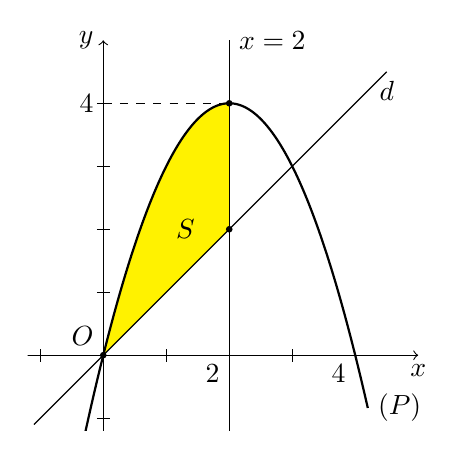
\begin{tikzpicture}[scale=0.8]
	\clip (-1.2,-1.2)rectangle(5.2,5.2);
	\draw[->] (-2,0)--(5,0)node[below]{$x$};
	\draw[->] (0,-2)--(0,5)node[left]{$y$};
	\fill[yellow](0,0)--plot[domain=0:2](\x,{-\x*(\x-4)})--(2,2)--cycle;
	\draw[dashed](0,4)--(2,4);
	\draw(2,-2)--(2,5)node[right]{$x=2$}; 
	\draw (-1.1,-1.1)--(4.5,4.5)node[below]{$d$};
	\draw[thick,samples=150,smooth,domain=-0.3:4.2] plot(\x,{-\x*(\x-4)})node[right]{$(P)$};
	\foreach \d in {2,4}{\path (\d,0)node[below left]{$\d$};}
	\foreach \d in {4}{\path (0,\d)node[left]{$\d$};}
	\foreach \i in{-1,1,3}{\draw(\i,-.1)--(\i, .1);}
	\foreach \i in{-1,1,2,3,4}{\draw(-.1,\i)--( .1,\i);}
	\foreach \t in {(0,0), (2,2), (2,4)}{\fill \t circle (1.5pt); }
	\path (0,0)node[above left]{$O$} (1,2)node[right]{$S$};
	\end{tikzpicture}
	\end{center}
	\choiceTF
	{\True $(P)$ và $d$ cắt nhau tại hai điểm phân biệt}
	{Dện tích $S_1$ của hình phẳng giới hạn bởi $(P)$, trục hoành và hai đường thẳng $x=0, x=2$ là $2$}
	{Dện tích $S_2$ của hình phẳng giới hạn bởi $d$, trục hoành và hai đường thẳng $x=0, x=2$ là $\dfrac{16}{3}$}
	{\True Diện tích $S$ của hình phẳng giới hạn bởi $(P), d$ và hai đường thẳng $x=0, x=2$ là $\dfrac{10}{3}$}
	\loigiai{
	\begin{itemchoice}
	\itemch $(P)$ và $d$ cắt nhau tại hai điểm phân biệt.
	\itemch Diện tích cần tìm là $S_1=\displaystyle\int\limits_{0}^{2} |4x-x^2|
	\mathrm{\,d}x$.\\
	Ta có: $4x-x^2\ge 0$ với mọi $x\in[0;2]$.\\
	Vậy $S_1=\displaystyle\int\limits_{0}^{2} |4x-x^2|
	\mathrm{\,d}x=\displaystyle\int\limits_{0}^{2} (4x-x^2)
	\mathrm{\,d}x=\left(2x^2-\dfrac{x^3}{3}\right)\bigg|_0^2=\dfrac{16}{3}$.
	\itemch Gọi $S_2$ là diện tích hình phẳng giới hạn bởi $d$, trục hoành và hai đường thẳng $x=0, x=2$.\\
	Vì $x\ge0$ với mọi $x\in[0;2]$ nên ta có\\
	$S_2=\displaystyle\int\limits_{0}^{2} |x|
	\mathrm{\,d}x=\displaystyle\int\limits_{0}^{2} x
	\mathrm{\,d}x=\dfrac{x^2}{2}\bigg|_0^2=2$.
	\itemch Diện tích cần tìm là $S=S_1-S_2=\dfrac{10}{3}$.
	\end{itemchoice}
	}
\end{ex}
%Câu 2
\begin{ex}%[2D4V3-2]
	Một chiếc cổng có hình dạng là một parabol $(P)$ có kích thước như hình vẽ, biết chiều cao cổng bằng $4$m, $AB=4$m. Người ta thiết kế cửa đi là một hình chữ nhật $CDEF$ (với $C,F\in AB;\ D,E\in (P)$), phần còn lại (\textit{phần tô đậm}) dùng để trang trí. Biết chi phí để trang trí phần tô đậm là $1\,000\,000$ đồng/m$^2$. Gắn hệ trục tọa độ $Oxy$ như hình bên dưới.
	\begin{center}
	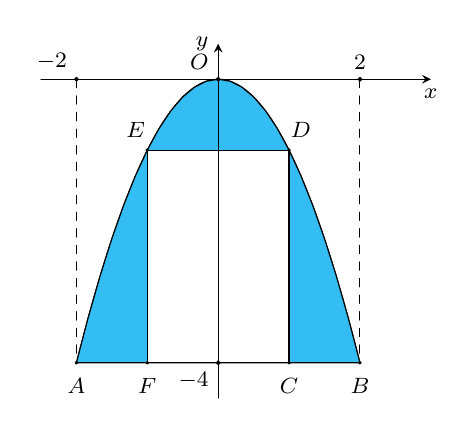
\begin{tikzpicture}[>=stealth,line join=round,line cap=round,font=\footnotesize,scale=.45]
	\path 
	(2,-2)coordinate(D)
	(-2,-2)coordinate(E)
	(2,-8)coordinate(C)
	(-2,-8)coordinate(F)
	(-4,-8)coordinate(A)
	(4,-8)coordinate(B)
	;
	\draw[smooth,samples=100,domain=-4:4] plot(\x,{-0.5*(\x)^2});
	\draw (C)--(D)--(E)--(F) (A)--(B);
	\draw[fill=cyan!80] (A) plot[domain=-4:4](\x,{-0.5*(\x)^2}) (B)--(A);
	\draw[fill=white] (C)--(D)--(E)--(F)--(C);
	\draw[->] (-5,0)--(6,0) node[below] {$x$};
	\draw[->] (0,-9)--(0,1) node[left] {$y$};
	\draw[fill=black] (0,0) node[above left=-0.1] {$O$} circle (1.5pt);
	\draw[fill=black] (0,-8) node[below left=-0.1] {$-4$} circle (1.5pt);
	\draw[fill=black] (-4,0) node[above left=-0.1] {$-2$} circle (1.5pt);
	\draw[fill=black] (4,0) node[above] {$2$} circle (1.5pt);
	\draw[dashed] (-4,0)--(-4,-8) (4,0)--(4,-8);
	\foreach \p/\g in {A/-90,F/-90,C/-90,B/-90,E/120,D/60}
	\draw[fill=black] (\p) circle (1pt) node[shift=(\g:3mm)] {$\p$};
	\end{tikzpicture}
	\end{center}
	\choiceTF
	{\True Parabol đi qua điểm $A(-2;4)$}
	{Phương trình của chiếc cổng parabol là $y=x^2$}
	{\True Diện tích cổng parabol (tính luôn cả cửa đi) là $\dfrac{32}{3}$}
	{Số tiền dùng để trang trí nhỏ nhất là $4\,000\,000$ đồng}
	\loigiai{
	\begin{itemchoice}
	\itemch Parabol đi qua điểm $A(-2;4)$
	\itemch Parabol có phương trình $y=ax^2+bx+c$.\\
	Parabol đi qua $3$ điểm $A(-2;-4)$, $O(0;0)$ và $B(2;-4)$ nên ta có
	$$\heva{&4a-2b+c=-4\\&4a+2b+c=-4\\&c=0}\Leftrightarrow\heva{&a=-1\\&b=0\\&c=0.}$$
	Khi đó, parabol có phương trình là $y=x^2$.
	\itemch Diện tích của hình phẳng giới hạn bởi parabol $(P)$ và đường thẳng $y=-4$ bằng
	$$S_1=\displaystyle\int\limits_{-2}^{2}\left|-x^2+4\right|\mathrm{d}x=\dfrac{32}{3}.$$
	\itemch Gọi $D\left(t,-t^2\right)\in(P)$ với $0<t<2$. Diện tích của hình chữ nhật $CDEF$ là\\
	\[S_2=2t\cdot \left(-t^2+4\right)=-2t^3+8t.\]
	Diện tích phần trang trí
	\[S=S_1-S_2=2t^3-8t+\dfrac{32}{3}.\]
	Để số tiền dùng để trang trí nhỏ nhất thì diện tích phần trang trí nhỏ nhất.\\
	Xét hàm $f(t)=2t^3-8t+\dfrac{32}{3}$ trên $(0;2)$. Ta có
	\[f'(t)=6t^2-8=0\Rightarrow t= \dfrac{2}{\sqrt{3}}.\]
	Bảng biến thiên
	\begin{center}
	
\begin{tikzpicture}[>=stealth]
	\tkzTabInit[lgt=1.5,espcl=2.5]
	{$t$ /1.2, $f'(t)$ /1, $f(t)$ /2}
	{$0$, $\dfrac{2}{\sqrt{3}}$, $2$}
	\tkzTabLine{,-,0,+,}
	\tkzTabVar{+/ $\dfrac{32}{3}$, -/ $f_{\text{CT}}$, +/ $\dfrac{32}{3}$}
	\end{tikzpicture}
	\end{center}
	Do đó, $\min\limits_{(0;2)}f(t)=f\left(\dfrac{2}{\sqrt{3}}\right)=\dfrac{96-32\sqrt{3}}{9}\approx 4{,}5083$.\\
	Vậy số tiền dùng để trang trí nhỏ nhất gần bằng	$4{,}508\cdot 1\,000\,000=4\,508\,000\ \text{đồng}.$
	\end{itemchoice}
	}
\end{ex}
%Câu 3
\begin{ex}%[2D4V3-5]
	Một thùng rượu vang có dạng khối tròn xoay với bán kính mặt đáy và mặt ở trên là $33$ cm, bán kính mặt cắt ở chính giữa thùng là $43$ cm. Chiều cao của thùng rượu là $112$ cm, bao gồm phần thân thùng rượu, hai đế đỡ thùng rượu (mỗi đế cao $3$ cm) và thùng rượu được ghép từ các thanh gỗ sồi với độ dày mỗi thanh gỗ là $3$ cm (Hình 1a). Hình 1b mô phỏng phần bên trong thùng rượu có dạng một khối tròn xoay tạo thành khi quay một phần của parabol $(P)\colon y=ax^2+bx+c$ quanh trục hoành (mỗi đơn vị ứng với $10$ cm).
	\begin{center}
	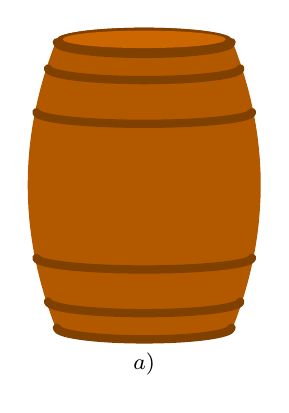
\begin{tikzpicture}[scale=0.37, font=\footnotesize, line join=round, line cap=round,>=stealth]
	\begin{scope}[rotate=90]
	\fill[orange!70!black, draw=none] (-5,-3)arc (-90:-270: 0.4 and 3)--(-5,3)--plot[domain=-5:5](\x,{-1/25*(\x)^2+4})--(5,3)arc (90:-90: 0.4 and 3)--(5,-3)--plot[domain=5:-5](\x,{1/25*(\x)^2-4})--cycle;
	\fill[orange!50!black,draw=none] (5,0) ellipse (0.4 and 3);
	\fill[orange!80!black,draw=none] (5,0) ellipse (0.3 and 2.8);
	\draw[color=orange!50!black,line width=3pt] (4.9,3) arc (90:270: 0.4 and 3);
	\draw[color=orange!50!black,line width=3pt] (4,3.3) arc (90:270: 0.4 and 3.3);
	\draw[color=orange!50!black,line width=3pt] (2.5,3.7) arc (90:270: 0.4 and 3.7);
	\draw[color=orange!50!black,line width=3pt] (-2.5,3.7) arc (90:270: 0.4 and 3.7);
	\draw[color=orange!50!black,line width=3pt] (-4,3.3) arc (90:270: 0.4 and 3.3);
	\draw[color=orange!50!black,line width=3pt] (-4.9,3) arc (90:270: 0.4 and 3);
	\end{scope}
	\node[below] at (current bounding box.south){$a)$};
	\end{tikzpicture}
	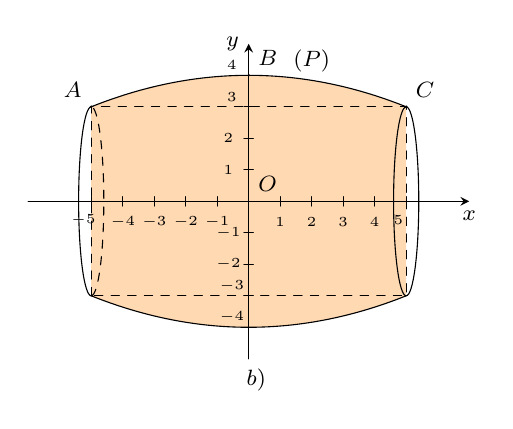
\begin{tikzpicture}[scale=0.4, font=\footnotesize, line join=round, line cap=round,>=stealth]
	\fill[color=orange!30, draw=none] (-5,-3)--(-5,3)--plot[domain=-5:5](\x,{-1/25*(\x)^2+4})--(5,3)--(5,-3)--plot[domain=5:-5](\x,{1/25*(\x)^2-4})--cycle;
	\draw[->] (-7,0) --(7,0) node[below]{$x$};
	\draw[->] (0,-5) --(0,5) node[left]{$y$};
	\draw (0,0) node[above right]{$O$};
	\draw[smooth,samples=200,domain=-5:5] plot(\x,{-1/25*(\x)^2+4});
	\draw[smooth,samples=200,domain=-5:5] plot(\x,{1/25*(\x)^2-4});
	\draw (5,0) ellipse (0.4 and 3);
	\draw (-5,3) arc (90:270: 0.4 and 3);
	\draw[dashed] (-5,-3) arc (-90:90: 0.4 and 3);
	\draw[dashed] (-5,-3)--(-5,3)--(5,3)--(5,-3)--cycle;
	\fill[color=black] 
	(-5,3) node[above left] {$A$} circle (1.25pt)
	(0,4) node[above right] {$B$} circle (1.25pt)
	(5,3) node[above right] {$C$} circle (1.25pt)
	(2,3.8) node[above] {$(P)$}
	;
	\foreach \x in {-2,-1,1,2}
	\draw (0.15,\x)--(-0.15,\x) node[shift={(180:2mm)},font=\tiny]{$\x$};
	\foreach \x in {-4,-3,3,4}
	\draw (0.15,\x)--(-0.15,\x) node[shift={(140:2mm)},font=\tiny]{$\x$};
	\foreach \x in {-4,-3,-2,-1,1,2,3,4}
	\draw (\x,0.15)--(\x,-0.15) node[shift={(-90:2mm)},font=\tiny]{$\x$};
	\foreach \x in {-5,5}
	\draw (\x,0.15)--(\x,-0.15) node[shift={(-120:2mm)},font=\tiny]{$\x$};
	\node[below] at (current bounding box.south){$b)$};
	\end{tikzpicture}
	\end{center}
\choiceTF
{\True Phần bên trong thùng rượu có chiều cao là $100$ cm}
{Hệ số $b=0$ và $c=20$}
{\True Parabol $(P)$ có phương trình $y=-\dfrac{1}{250}x^2+40$}
{\True Thùng rượu đó chứa được tối đa $425{,}16$ lít rượu (làm tròn kết quả đến hàng phần trăm)}
	\loigiai{
	\begin{itemchoice}
	\itemch Chiều cao bên trong của thùng rượu là $112-3\cdot 4=100$ (cm).
	\itemch Parabol $(P)$ có đỉnh $B(0;40)$ nên $b=0$, $c=40$.
	\itemch Mặt khác $(P)$ đi qua $C(50;30)$ nên suy ra
	$$ 30=a\cdot 50^2+0\cdot 50+40\Leftrightarrow 2500 a=-10\Leftrightarrow a=-\dfrac{1}{250}. $$
	Vậy $a=-\dfrac{1}{250}$, $b=0$, $c=40$.
	\itemch Thể tích thùng rượu (tính bằng đơn vị $\mathrm{cm}^3$) bằng thể tích khối tròn xoay tạo thành khi quay quanh $Ox$ hình phẳng giới hạn bởi $(P)$, trục $Ox$ và hai đường thẳng $x=-50$, $x=50$. Vậy số lít rượu tối đa mà thùng rượu chứa được là
	$$ V=\dfrac{1}{1000}\cdot \pi \int\limits_{-50}^{50} \left(-\dfrac{1}{250}x^2+40\right)^2\,\mathrm{d}x=\dfrac{406\pi}{3}\approx 425{,}16\quad (\text{lít}). $$
	\end{itemchoice}
	}
\end{ex}
%Câu 4
\begin{ex}%[2D4V3-2]
Trên cửa sổ có dạng hình chữ nhật, hoạ sĩ thiết kế logo hình con cá cho một doanh nghiệp kinh doanh hải sản. Logo là hình phẳng giới hạn bởi hai parabol với các kích thước được cho trong hình bên (đơn vị trên mỗi trục toạ độ là dm).
\begin{center}
		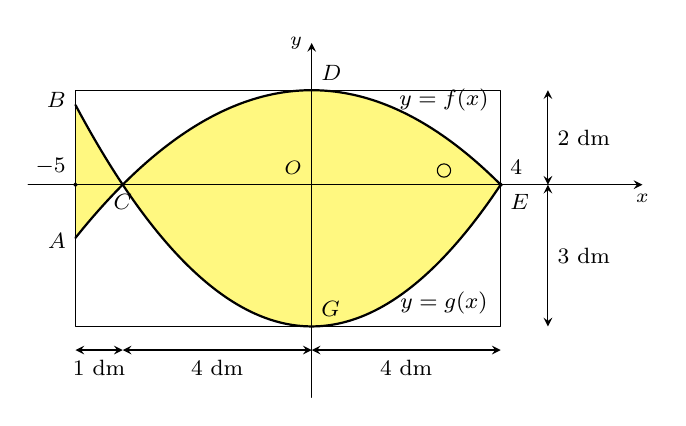
\begin{tikzpicture}[line join = round, line cap = round,>=stealth,font=\footnotesize,scale=0.6]
	\def \xmin{-6}
	\def \ymin{-4.5}
	\def \xmax{7}
	\def \ymax{3}
	\fill[yellow!50,smooth] plot[domain=-5:4] (\x,{-0.125*(\x)^2+2})-- (4,0) -- plot[domain=4:-5] (\x,{0.1875*(\x)^2-3}) -- (-5,-1.125);
	\draw[->] (\xmin,0) -- (\xmax,0) node[below] {\scriptsize $x$};
	\draw[->] (0,\ymin) -- (0,\ymax) node[left] {\scriptsize $y$};
	\clip (\xmin+0.1,\ymin+0.1) rectangle (\xmax-0.1,\ymax-0.1);
	\draw (0,0) node[above left]{\scriptsize $O$};
	\draw[thick,samples=150,smooth,domain=-5:4] plot(\x,{-0.125*(\x)^2+2});
	\draw[thick,samples=150,smooth,domain=-5:4] plot(\x,{0.1875*(\x)^2-3});
	\draw[fill=black] (4,0) circle(1pt) node[above right]{$4$} (-5,0) circle(1pt) node[above left]{$-5$};
	\draw (2.8,0.3) circle (4pt);
	\path 
	(4,0) coordinate (O)
	(2,1.5) coordinate (A)
	;
	\draw (-5,-3) rectangle (4,2);
	\draw (2.8,-2.5) node {$y=g(x)$};
	\draw (2.8,1.8) node {$y=f(x)$};
	\draw (-4,0) node[below] {$C$};
	\draw (-5,-1.2) node[left] {$A$};
	\draw (-5,1.8) node[left] {$B$};
	\draw (4,0) node[below right] {$E$};
	\draw (0,2) node[above right] {$D$};
	\draw (0,-3) node[above right] {$G$};
	\draw[<->] (5,0) -- (5,2);
	\draw (5,1) node[right] {$2$ dm};
	\draw[<->] (5,0) -- (5,-3);
	\draw (5,-1.5) node[right] {$3$ dm};
	\draw[<->] (-5,-3.5) -- (-4,-3.5);
	\draw (-4.5,-3.5) node[below] {$1$ dm};
	\draw[<->] (-4,-3.5) -- (0,-3.5);
	\draw (-2,-3.5) node[below] {$4$ dm};
	\draw[<->] (0,-3.5) -- (4,-3.5);
	\draw (2,-3.5) node[below] {$4$ dm};
	\end{tikzpicture}
\end{center}
\choiceTF
{\True Diện tích logo được tính theo công thức $\displaystyle\int\limits_{-5}^{4} \left|f(x)-g(x)\right| \mathrm{\,d}x$}
{\True Phương trình $f(x)=-\dfrac{1}{8}x^2+2$}
{Phương trình $g(x)=\dfrac{3}{16}x^2+3$}
{Diện tích của logo là $\dfrac{1354}{48}$ dm$^2$}
	\loigiai
	{
	\begin{itemchoice}
	\itemch Diện tích logo là $S=\displaystyle\int\limits_{-5}^{4} \left|f(x)-g(x)\right| \mathrm{\,d}x$.
	\itemch Giả sử parabol $y=f(x)$ cho bởi công thức $f(x)=ax^2+bx+c$ ($a\neq 0$).\\
	Do parabol $y=f(x)$ đi qua điểm $D(0;2)$ nên $c=2$, suy ra $f(x)=ax^2+bx+2$ ($a\neq 0$).\\
	Vì parabol $y=f(x)$ đi qua các điểm $C(-4;0)$ và $E(4;0)$ nên ta có hệ
	\begin{align*}
	\heva{& 16a-4b+2=0 \\ & 16a+4b+2=0}\Leftrightarrow \heva{& a=-\dfrac{1}{8} \\ & b=0.}
	\end{align*}
	Vậy $f(x)=-\dfrac{1}{8}x^2+2$.
	\itemch Giả sử parabol $y=g(x)$ cho bởi $g(x)=a_1x^2+b_1x+c_1$ ($a_1\neq 0$). Do parabol $y=g(x)$ đi qua điểm $G(0;-3)$ nên $c_1=-3$, suy ra $g(x)=a_1x^2+b_1x-3$ ($a_1\neq 0$). Vì parabol $y=g(x)$ đi qua các điểm $C(-4;0)$ và $E(4;0)$ nên ta có
	\begin{align*}
	\heva{& 16a_1-4b_1-3=0 \\ & 16a_1+4b_1-3=0}\Leftrightarrow \heva{& a_1=\dfrac{3}{16} \\ & b_1=0.}
	\end{align*}
	Vậy $g(x)=\dfrac{3}{16}x^2-3$.
	\itemch Diện tích của logo là $S=S_1+S_2$, trong đó $S_1$ là diện tích hình phẳng giới hạn bởi các parabol $f(x)=-\dfrac{1}{8}x^2+2$, $g(x)=\dfrac{3}{16}x^{2}-3$ và hai đường thẳng $x=-5$, $x=-4$; $S_2$ là diện tích hình phẳng giới hạn bởi các parabol $f(x)=-\dfrac{1}{8}x^2+2$, $g(x)=\dfrac{3}{16}x^2-3$ và hai đường thẳng $x=-4$, $x=4$.\\
	Do đó ta có
	\begin{eqnarray*}
	S&=&\displaystyle\int\limits_{-5}^{-4} \left|f(x)-g(x)\right| \mathrm{\,d}x+\displaystyle\int\limits_{-4}^{4} \left|f(x)-g(x)\right| \mathrm{\,d}x\\
	&=&\displaystyle\int\limits_{-5}^{-4} \left[g(x)-f(x)\right] \mathrm{\,d}x+\displaystyle\int\limits_{-4}^{4} \left[f(x)-g(x)\right] \mathrm{\,d}x\\
	&=&\displaystyle\int\limits_{-5}^{-4} \left[\left(\dfrac{3}{16}x^2-3\right)-\left(-\dfrac{1}{8}x^2+2\right)\right] \mathrm{\,d}x+\displaystyle\int\limits_{-4}^{4} \left(-\dfrac{1}{8}x^2+2\right)-\left(\dfrac{3}{16}x^2-3\right) \mathrm{\,d}x\\
	&=&\displaystyle\int\limits_{-5}^{4} \left(\dfrac{5}{16}x^2-5\right) \mathrm{\,d}x+\displaystyle\int\limits_{-4}^{4} \left(-\dfrac{5}{16}x^2+5\right) \mathrm{\,d}x\\
	&=&\dfrac{5}{48}x^3\bigg|_{-5}^{-4}-5x\bigg|_{-5}^{-4}-\dfrac{5}{48}x^3\bigg|_{-4}^4+5x\bigg|_{-4}^4\\
	&=&\dfrac{305}{48}-5-\dfrac{640}{48}+40=\dfrac{1345}{48}.
	\end{eqnarray*}
	\end{itemchoice}
	}
\end{ex}
\Closesolutionfile{ans}
% \indapan{3}{ans/ans-2-B13-1-DS}
\Opensolutionfile{ans}[ans/ans-2-B13-1-KQ]
\caukq
%Câu 1
\begin{ex}%[2D4H3-1]
	Gọi $S$ là hình phẳng giới hạn bởi đồ thị hàm số $(H)\colon y=\dfrac{x-1}{x+1}$ và các trục tọa độ. Tính diện tích hình phẳng $(S)$ (làm tròn đến chữ số thứ hai sau dấu phẩy).
	\shortans{$0{,}39$}
	\loigiai{
	Điều kiện $x\ne -1$.\\
	Hoành độ giao điểm của đồ thị hàm số và trục $Ox$ là nghiệm của phương trình $$\dfrac{x-1}{x+1}=0\Leftrightarrow x=1.$$
	Vậy diện tích hình phẳng cần tìm là 
	\allowdisplaybreaks
	\begin{eqnarray*}
	S&=&\displaystyle\int\limits_0^1 \left|\dfrac{x-1}{x+1}\right| \mathrm{\,d}x=\displaystyle\int\limits_0^1 \dfrac{1-x}{x+1} \mathrm{\,d}x
	=\displaystyle\int\limits_0^1 \left(-1+\dfrac{2}{x+1}\right) \mathrm{\,d}x\\
	&=&\left(-x+2\ln|x+1|\right)\Bigr\rvert_0^1=2\ln 2-1\approx 0{,}39.
	\end{eqnarray*}
	}
\end{ex}
%Câu 2
\begin{ex}%[2D4H3-3]
	Tính thể tích của khối tròn xoay khi cho hình phẳng giới hạn bởi đường thẳng $y=3x+2$ và đồ thị hàm số $y=2x^2$ quay quanh trục $Ox$ (làm tròn đến chữ số thứ nhất sau dấu phẩy).
	\shortans{$98{,}2$}
	\loigiai
	{
	Xét phương trình hoành độ giao điểm của hai đồ thị hàm số ta có \[2x^2=3x+2\Leftrightarrow\hoac{& x=-\dfrac{1}{2}\\&x=2. }\]
	Thể tích của khối tròn xoay cần tìm là
	\[V=\pi\displaystyle\int\limits_{-\tfrac{1}{2}}^{2}\left |\left (2x^2 \right )^2-(3x+2)^2 \right |=\dfrac{125\pi}{4}\approx98{,}2.\]
	}
\end{ex}
%Câu 3
\begin{ex}%[2D4V3-4]
	\immini{Cho vật thể đáy là hình tròn có bán kính bằng $1$ (tham khảo hình vẽ). Khi cắt vật thể bằng mặt phẳng vuông góc với trục $Ox$ tại điểm có hoành độ $x\ (-1\leq x\leq 1)$ thì được thiết diện là một tam giác đều. Tính thể tích vật thể đó (làm tròn đến chữ số đầu tiên sau dấu phẩy).\shortans{$2{,}3$}
	}{
	\begin{tikzpicture}[line cap=round,line join=round,scale=.6,font=\footnotesize,>=stealth]
	\def\h{4}
	\def\a{3}
	\def\x{.65}
	\pgfmathsetmacro\b{\a/3}
	\pgfmathsetmacro{\g}{asin(\b/\h)}
	\pgfmathsetmacro\xo{\a *cos(\g)}
	\pgfmathsetmacro\yo{\b *sin(\g)}
	\fill[draw,thick,top color=gray!15,bottom color=gray,smooth] (90:\h)coordinate(S)--(-\xo,\yo)coordinate(A) arc (180-\g:360+\g:{\a} and {\b})--(\x,{-(\x)^2+\h}) plot[domain=\x:0](\x,{-(\x)^2+\h});
	\begin{scope}
	\clip (90:\h)--(-\xo,\yo) arc (180-\g:360+\g:{\a} and {\b})--(\x,{-(\x)^2+\h}) plot[domain=\x:0](\x,{-(\x)^2+\h});
	\draw[smooth,thick] plot[domain=0:\a](\x,{-(\x)^2+\h});
	\foreach \x in {.1,.2,...,\a}\draw[opacity=.5] (\x,{-(\x)^2+\h})--++(-128:2*\h);
	\foreach \y in {-10,...,30}\draw[smooth,shift={($($(S)!\y/25!(A)$)-(S)$)},opacity=.5] plot[domain=0:\a](\x,{-(\x)^2+\h});
	\foreach \x in {.65,.75,...,\a}\draw[opacity=.5] (\x,{-(\x)^2+\h})--++(-55:\h);
	\end{scope}
	\end{tikzpicture}}
	\loigiai{
	\immini{
	Ta có $\triangle OAB$ đều có cạnh $AB=2AH=2\sqrt{1-x^2}.$\\
	Diện tích thiết diện là $S(x)=\dfrac{AB^2\cdot\sqrt{3}}{4}=\sqrt{3}\left(1-x^2\right)$.\\
	Khi đó thể tích vật thể là
	\allowdisplaybreaks
	\begin{eqnarray*}
	V&=& \displaystyle\int\limits_{-1}^1 S(x) \mathrm{\,d}x=\sqrt{3}\displaystyle\int\limits_{-1}^1 (1-x^2) \mathrm{\,d}x\\
	&=&\sqrt{3}\left(x-\dfrac{x^3}{3}\right)\bigg|_{-1}^1=\dfrac{4\sqrt{3}}{3}\approx 2{,}3.
	\end{eqnarray*}
	}{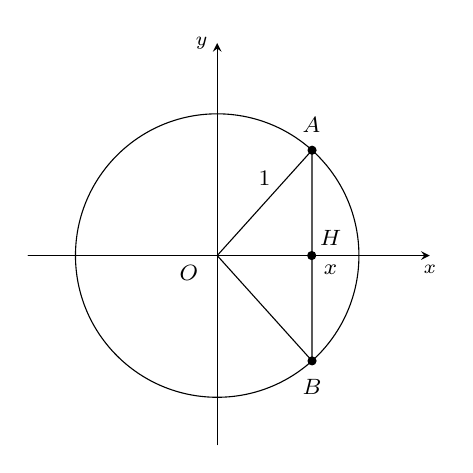
\begin{tikzpicture}[scale=1.2, font=\footnotesize,line join=round, line cap=round, >=stealth];
	\draw[->] (-2,0) -- (2.25,0) node[below] {\scriptsize $x$};
	\draw[->] (0,-2) -- (0,2.25) node[left] {\scriptsize $y$};
	\draw (-0.3,0) node[below] {$O$};
	\draw (60:1.6) node[right]{$A$};
	\draw (-60:1.6) node[right]{$B$};
	\draw (0:1.5) arc (0:360:1.5);
	\draw (0:0)--(48:1.5) (0:0)--(-48:1.5) (-48:1.5)--(48:1.5);
	\draw[fill=black] (48:1.5) circle (1.2pt) (-48:1.5) circle (1.2pt) (1,0) circle (1.2pt);
	\draw (1.2,0) node[below] {$x$};
	\draw (1.2,0) node[above] {$H$};
	\draw (0.5,1) node[below] {$1$};
	\end{tikzpicture}}
	}
\end{ex}
%Câu 4
\begin{ex}%[2D4V3-2]
	\immini
	{
	Một gia đình muốn làm cánh cổng (như hình vẽ). Phần phía trên cổng có hình dạng là một parabol với $IH=2{,}5$ m, phần phía dưới là một hình chữ nhật kích thước cạnh là $AD=4$ m, $A B=6$ m. Giả sử giá để làm phần cổng được tô màu là $1\,000\,000 \text{~đồng} / \mathrm{m}^2$ và giá để làm phần cổng phía trên là $1\,200\,000 \text{~đồng} / \mathrm{m}^2$. Số tiền tổng cộng gia đình cần trả là bao nhiêu triệu đồng?
	\shortans{$36$}
	}
	{
	\begin{tikzpicture}[scale=0.6, font=\footnotesize, line join=round, line cap=round, >=stealth]
	\draw (-3,-2.5) parabola bend (0,0) (3,-2.5);
	\fill (0,0)coordinate (I) circle (1pt) node[above]{$I$};
	\fill (0,-2.5)coordinate (H) circle (1pt) node[above right]{$H$};
	\fill (-3,-2.5)coordinate (A) circle (1pt) node[left]{$A$};
	\fill (3,-2.5)coordinate (B) circle (1pt) node[right]{$B$};
	\fill (-3,-6.5)coordinate (D) circle (1pt) node[left]{$D$};
	\fill (3,-6.5)coordinate (C) circle (1pt) node[right]{$C$};
	\draw (I)--(H) node[midway, right]{$2{,}5$ m};
	\draw (A)--(D) node[midway, left]{$4$ m};
	\draw (D)--(C) node[midway, below]{$6$ m};
	\draw[pattern = north east lines] (-3,-2.5) rectangle (3,-6.5);
	\end{tikzpicture}
	}
	\loigiai{
	\begin{center}
	\begin{tikzpicture}[scale=0.8, font=\footnotesize, line join=round, line cap=round, >=stealth]
	\draw (-3,-2.5) parabola bend (0,0) (3,-2.5);
	\draw (-11,-2.5) parabola bend (-8,0) (-5,-2.5);
	\draw[->] (-8,-5)--(-8,1)node[right]{$y$};
	\draw[->] (-12,0)--(-4,0)node[above]{$x$};
	\fill (-8,0) circle (1pt) node[above right]{$O$};
	\fill (-11,-2.5) circle (1.5pt) node[left]{$A$};
	\fill (-5,-2.5) circle (1.5pt) node[right]{$B$};
	\draw[dashed] (-11,0)--(-11,-2.5)--(-8,-2.5);
	\draw[dashed] (-5,0)--(-5,-2.5)--(-8,-2.5);
	\fill (0,0)coordinate (I) circle (1pt) node[above]{$I$};
	\fill (0,-2.5)coordinate (H) circle (1pt) node[above right]{$H$};
	\fill (-3,-2.5)coordinate (A) circle (1pt) node[left]{$A$};
	\fill (3,-2.5)coordinate (B) circle (1pt) node[right]{$B$};
	\fill (-3,-6.5)coordinate (D) circle (1pt) node[left]{$D$};
	\fill (3,-6.5)coordinate (C) circle (1pt) node[right]{$C$};
	\draw (I)--(H) node[midway, right]{$2.5$ m};
	\draw (A)--(D) node[midway, left]{$4$ m};
	\draw (D)--(C) node[midway, below]{$6$ m};
	\draw[pattern = north east lines] (-3,-2.5) rectangle (3,-6.5);
	\fill (-11,0) circle (1pt) node[above]{$-3$};
	\fill (-5,0) circle (1pt) node[above]{$3$};
	\fill (-8,-2.5) circle (1pt) node[below left]{$-2{,}5$};
	\end{tikzpicture}
	\end{center}
	Diện tích hình chữ nhật $ABCD$ là $S_{ABCD}=24 \text{~m}^2$.\\
	Chọn hệ trục toạ độ như hình vẽ. Khi đó Parabol đi qua $3$ điểm $A$, $O$, $B$ có dạng $(P)\colon y=ax^2$.\\
	Mặt khác $B(3;-2{,}5)\in (P)\Rightarrow 9a=-2{,}5\Leftrightarrow a=-\dfrac{5}{18}$.\\
	Do đó $(P)\colon y=-\dfrac{5x^2}{18}$.\\
	Diện tích cổng hình Parabol là $$S=\displaystyle\int\limits_{-3}^3 \left[ \left( -\dfrac{5x^2}{18}\right)-(-2{,}5)\right] \mathrm{\,d}x=\left( -\dfrac{5x^3}{54}+\dfrac{5x}{2}\right) \bigg|_{-3}^3=10.$$
	Vậy tổng số tiền làm cổng là $T=24\cdot 1\,000\,000+10\cdot 1\,200\,000=36$ triệu đồng.
	}
\end{ex}
%Câu 5
\begin{ex}%[2D4C3-1]
	\immini{
	Cho hai hàm số $f(x)=ax^3+bx^2+cx-1$ và $g(x)=dx^2+ex+\dfrac{1}{2}$ với $(a,b,c,d\in\mathbb{R})$. Biết đồ thị của hàm số $y=f(x)$ và $y=g(x)$ cắt nhau tại ba điểm có hoành độ lần lượt là $-3$, $-1$, $2$ (tham khảo hình vẽ bên). Tính diện tích hình phẳng giới hạn bởi hai đồ thị đã cho (làm tròn đến chữ số đầu tiên sau dấu phẩy).\par\shortans{$5{,}3$}
	}
	{\begin{tikzpicture}[scale=0.6, font=\footnotesize, line join=round, line cap=round, >=stealth]
	\def\xt{-4} \def\xp{3} \def\yd{-2} \def\yt{5}
	\draw[->](\xt,0) -- (0,0)node[below right]{$O$} -- (\xp,0)node[below]{$x$};
	\draw[->](0,\yd)--(0,\yt)node[left]{$y$};
	\begin{scope}
	\clip (\xt,\yd) rectangle (\xp,\yt);
	\draw[smooth,samples=150] plot[domain=\xt:\xp](\x,{0.25*(\x)^3+0.75*(\x)^2-0.75*(\x)-1});
	\draw[smooth,samples=150] plot[domain=\xt:\xp](\x,{0.25*(\x)^2+0.5*(\x)+0.5});
	\fill[pattern=north west lines] plot[smooth,samples=100,domain=-3:-1] (\x,{0.25*(\x)^3+0.75*(\x)^2-0.75*(\x)-1})--plot[smooth,samples=100,domain=-1:-3] (\x,{0.25*(\x)^2+0.5*(\x)+0.5});
	\fill[pattern=north west lines] plot[smooth,samples=100,domain=-1:2] (\x,{0.25*(\x)^2+0.5*(\x)+0.5})--plot[smooth,samples=100,domain=2:-1] (\x,{0.25*(\x)^3+0.75*(\x)^2-0.75*(\x)-1});
	\end{scope}
	\draw[dashed] (-3,0) -- (-3,1.25) (-1,0)--(-1,0.25) (2,0)--(2,2.5);
	\foreach \i in {(0,0),(-3,0),(-1,0),(2,0),(-3,1.25),(-1,0.25),(2,2.5)} \fill \i circle(1pt);
	\path
	(-3,0) node[below]{$-3$}
	(-1,0) node[below]{$-1$}
	(2,0) node[below]{$2$};
	\end{tikzpicture}
	}
	\loigiai{
	Do đồ thị của hàm số $y=f(x)$ và $y=g(x)$ cắt nhau tại ba điểm có hoành độ lần lượt là $-3$, $-1$, $2$ nên suy ra
	\allowdisplaybreaks
	\begin{eqnarray*}
	&&f(x)-g(x)=ax^3+\left(b-d\right)x^2+\left(c-e\right)x-\dfrac{3}{2}
	=a\left(x+3\right)\left(x+1\right)\left(x-2\right)=a(x^3+2x^2-5x-6).
	\end{eqnarray*}
	Đồng nhất hệ số ta có $-6a=-\dfrac{3}{2}\Rightarrow a=\dfrac{1}{4}$.\\
	Khi đó diện tích hình phẳng bằng
	\allowdisplaybreaks
	\begin{eqnarray*}
	V&=&\displaystyle\int\limits_{-3}^2\left|f(x)-g(x)\right|\mathrm{\,d}x=\displaystyle\int\limits_{-3}^{-1}\left(f(x)-g(x)\right)\mathrm{\,d}x+\displaystyle\int\limits_{-1}^2\left(g(x)-f(x)\right)\mathrm{\,d}x\\
	&=&\displaystyle\int\limits_{-3}^{-1}\dfrac{1}{4}\left(x^3+2x^2-5x-6\right)\mathrm{\,d}x-\displaystyle\int\limits_{-1}^{2}\dfrac{1}{4}\left(x^3+2x^2-5x-6\right)\mathrm{\,d}x\\
	&=&\dfrac{1}{4}\left(\dfrac{1}{4}x^4+\dfrac{2}{3}x^3-\dfrac{5}{2}x^2-6x\right)\Bigg|_{-3}^{-1}-\dfrac{1}{4}\left(\dfrac{1}{4}x^4+\dfrac{2}{3}x^3-\dfrac{5}{2}x^2-6x\right)\Bigg|_{-1}^{2}\\
	&=&\dfrac{4}{3}+\dfrac{63}{16}=\dfrac{253}{48}.
	\end{eqnarray*}
	}
\end{ex}
%Câu 6
\begin{ex}%[2D4C3-3]
	\immini{
	Một vật trang trí có dạng một khối tròn xoay được tạo thành khi xoay miền $(R)$ (phần gạch chéo trong hình vẽ bên) quanh trục $AB$. Miền $(R)$ được giới hạn bởi các cạnh $AB$, $AD$ của hình vuông $ABCD$ và các cung phần tư của các đường tròn bán kính bằng $1$ cm với tâm lần lượt là trung điểm của các cạnh $BC$, $AD$. Tính thể tích của vật trang trí đó (đơn vị cm$^3$), làm tròn kết quả đến hàng phần mười.
	\par\shortans{$10{,}5$}
	}{
	\begin{tikzpicture}[scale=0.6]
	\coordinate (A) at (0,0);
	\coordinate (B) at (0,-4);
	\coordinate (C) at (4,-4);
	\coordinate (D) at (4,0);
	\draw (A)--(B)--(C)--(D)--(A);
	\draw[pattern=north east lines] (B) arc (180:90:2) arc (-90:0:2)--(A)--(B);
	\path node at (A) [above left]{$A$}
	node at (B) [below left] {$B$}
	node at (C) [below right] {$C$}
	node at (D) [above right] {$D$};
	\end{tikzpicture}
	}
	\loigiai{
	\begin{center}
	\begin{tikzpicture}[scale=0.85]
	\draw [->] (0,-4) --(5,-4);
	\draw [->] (0,-4) --(0,1);
	\coordinate (D) at (0,0);
	\coordinate (A) at (0,-4);
	\coordinate (B) at (4,-4);
	\coordinate (C) at (4,0);
	\coordinate (I) at (4,-2);
	\coordinate (J) at (0,-2);
	\coordinate (K) at (2,-2);
	\draw (A)--(B)--(C)--(D)--(A);
	\draw[pattern=north west lines,opacity=0.4] (D) arc (90:0:2) arc (180:270:2)--(B)--(A)--(D);
	\foreach \x in {A,B,C,D,I,J,K}{
	\fill (\x) circle (1pt);
	}
	\draw[line width=1.5pt, red] (D) arc (90:0:2);
	\draw[dashed, opacity=0.4,red] (D) arc (90:450:2); 
	\draw[line width=1.5pt, blue] (K) arc (180:270:2);
	\draw[dashed, opacity=0.4,blue] (K) arc (180:540:2);
	\path node at (D) [above left]{$D$}
	node at (A) [below left] {$A\equiv O$}
	node at (B) [below right] {$B$}
	node at (C) [above right] {$C$}
	node at (I) [left] {$I$}
	node at (J) [left] {$J$}
	node at (5,-4) [below] {$x$}
	node at (0,1) [left] {$y$}
	node at (K) [right] {$K$}
	node at (2.6,-0.3) {$y=1+\sqrt{1-x^2}$}
	node at (4.2,-3) {$y=1-\sqrt{1-(x-2)^2}$};
	\end{tikzpicture}
	\end{center}
	Ta xoay hình lại và đưa vào hệ trục tọa độ như trên hình vẽ. Khi đó phần gạch chéo trên hình sẽ quay quanh trục $Ox$.\\
	Đường tròn tâm $J$
	\allowdisplaybreaks
	\begin{eqnarray*}
	x^2+(y-1)^2=1&\Rightarrow& (y-1)^2=1-x^2\\
	& \Leftrightarrow& |y-1|=\sqrt{1-x^2}\\
	& \Leftrightarrow &\heva{& y-1 =\sqrt{1-x^2}, \mbox{ khi } y\ge 1 \\& -(y-1) =\sqrt{1-x^2}, \mbox{ khi } y< 1} \\
	&\Leftrightarrow& \heva{& y =1+\sqrt{1-x^2}, \mbox{ khi } y\ge 1 \\& y=1-\sqrt{1-x^2} , \mbox{ khi } y< 1.}
	\end{eqnarray*}	
	Suy ra đồ thị đường cong từ $D$ đến $K$ là $y=1+\sqrt{1-x^2}$ với $x\in [0;1]$.\\	
	Đường tròn tâm $I$
	\begin{eqnarray*}
	(x-2)^2+(y-1)^2=17&\Rightarrow& (y-1)^2=1-(x-2)^2 \\
	&\Leftrightarrow& |y-1|=\sqrt{1-(x-2)^2}\\
	&\Leftrightarrow& \heva{& y-1 =\sqrt{1-(x-2)^2}, \mbox{ khi } y\ge 1 \\& -(y-1) =\sqrt{1-(x-2)^2}, \mbox{ khi } y< 1}\\
	&\Leftrightarrow& \heva{& y =1+\sqrt{1-(x-2)^2}, \mbox{ khi } y\ge 1 \\& y=1-\sqrt{1-(x-2)^2} , \mbox{ khi } y< 1}
	\end{eqnarray*}
	Suy ra đồ thị đường cong từ $K$ đến $B$ là $y=1-\sqrt{1-(x-2)^2}$ với $x\in [1;2]$.\\	
	Đường cong đi từ $D$ đến $B$ trên hình gồm hai phần$\colon$ phần thứ nhất là một phần tư đường tròn đi từ $D$ đến $K$ của đường tròn tâm $J$ và phần thứ hai là một phần tư đường tròn đi từ $K$ đến $B$ của đường tròn tâm $I$.\\
	Thể tích của vật trang trí là
	$$V= \pi\displaystyle\int\limits_0^1 \left(1+\sqrt{1-x^2}\right)^2\mathrm{\,d}x + \pi\displaystyle\int\limits_1^2 \left(1-\sqrt{1-(x-2)^2}\right)^2\mathrm{\,d}x \approx 10{,}5 \mbox{ cm}^3.$$
	}
\end{ex}
\Closesolutionfile{ans}